%!TEX root = RadioPaper_Main.tex
The following section describes the evaluation procedure applied to the proposed algorithm. 
%Results in this section are based on the predicted values $\hat{r}_m$ from (\ref{eq:prediction}), without applying any heuristics.
%For the results, all tracks are considered and picked exactly according to the ranking induced by $\hat{r}_m$ \footnote{\todo{
%We may have to add a footnote that in a production system, there might be additional interleaving and small heuristics, which of course
%we can't explain here. It's both outside the scope of the paper, and the secret in the sauce. Or something like that.
%}}.
%We first provide evidence that personalization is essential to quality in our learning problem. Next we illustrate the importance of different features we used. Finally, we show how our model handles well the ``cold start" problem.

\subsection{Datasets}
As explained in Section~\ref{sec:playlist_is_classification}, the model in this paper treats playlist generation
as a classification problem, for which the parameters can be
learned from examples, judiciously labeled through a variety of approaches.
The  two datasets  used for the evaluations exemplify different approaches to the construction of the training data:

\noindent{\bf Groove Music Dataset}
is a proprietary dataset of user preferences that was collected anonymously from Microsoft's Groove music service.
It contains 334,120 users, 472,908 tracks from 45,239 artists categorized into 100 sub-genres from 17 genres. Positive labels
are assigned to tracks in a user's listening history that were heard to completion. Negative labels are assigned to tracks that were skipped in mid-play by the user.

\noindent{\bf 30Music Dataset}
is a publicly available dataset of user playlists \cite{DBLP:conf/recsys/TurrinQCPC15}. Tracks in this dataset were intersected with Groove's catalog in order to enable feature generation (i.e. audio and content features). The resulting dataset contains 14,185 users, 252,424 tracks from 63,314 artists categorized into 99 sub-genres from 17 genres. Positive labels are assigned to tracks appearing in a user's playlist. Since no skip information was available, negatively labeled examples were obtained by uniformly sampling from tracks that did not appear in the user's playlist.
% \end{enumerate}


\subsection{Experimental Setup and Results}
We quantify the quality of the model using the \textit{Area Under Curve} (AUC) metric \cite{AUCRef}. AUC enables quantifying the trade-off between true positives and false positives over a range of threshold configurations. By doing so, AUC captures the overall quality of a particular prediction method.

%More formally, AUC is given by the following expression over threshold $t$:
%%%
%$$
%\mathrm{AUC} = \int_0^1 \mathrm{TPR}(t) \, \mathrm{FPR'}(t) \, d t
%$$
%%%
%where $\mathrm{FPR}(t)$ and $\mathrm{TPR}(t)$ are the True- and False Positive Rates at threshold $t$ respectively. %(TPR and FPR) are:

%\noam{We need to save space, so assume the reader known TPR and FPR.}
%%%
%\begin{align*}
%\mathrm{TPR}(t) & = \frac{1}{|\mathcal{X}_{\mathrm{pos}} |}
%\sum_{\x \in \mathcal{X}_{\mathrm{pos}}} \mathbb{I} \Big[ \widetilde{p}_{\phi}(r = 1 | \x, \mathcal{D}, \mathcal{H} ) \geq t \Big] \\
%\mathrm{FPR}(t) & = \frac{1}{|\mathcal{X}_{\mathrm{neg}} |}
%\sum_{\x \in \mathcal{X}_{\mathrm{neg}}} \mathbb{I} \Big[ \widetilde{p}_{\phi} (r = 1 | \x, \mathcal{D}, \mathcal{H} ) \geq t \Big] \ .
%\end{align*}
%%%
%$\mathcal{X}_{\mathrm{pos}}$ and $\mathcal{X}_{\mathrm{neg}}$ denote the subset of positive and negatively labeled examples, respectively, of an evaluation set with known labels, while $\phi$ indexes a particular subset of parameters, and
%$\widetilde{p}_{\phi} \in [0,1]$ denotes the probability given by (\ref{eq:PredictionApproximation}).
%\todo{the equation below (\ref{eq:prediction})} 
%The following section outlines the models tested.
%\todo{we have to tidy up notation and write TPR in terms of our actual model. I put a tilde over the $p$ to show that it's an
%approximation, but we can choose anything (and define it earlier). We also have to find a clean way to enumerate ``model'' in our
%notation, and allude to it earlier.}
%\GL{To ulrich's comment above: I added a definiton indexed on the parameter subset denoted $\phi$ in my notation in the last paragraph of the prediction sub-section}
%\todo{I removed threshold $\theta$ here and made it a $t$, so as not to overload symbols.}
%
%% $f\left(x\right) \in [0,1]$ denotes the confidence of the learned classifier.
%
%\todo{In (\ref{eq:prediction}) there should be no $\btheta$ in
%$p(r = 1 | \x, \mathcal{D}, \mathcal{H} )$, as we average over the posterior of $\btheta$ / integrate it out.}

%\subsection{Experimental Procedure}

The model was trained on 70\% of the examples and evaluated on the remaining 30\%. \GLw{We may have more results using cross-validation later in the week, so we can claim a stronger experimental setup}
%In what follows, the full model described in this paper is dubbed as {\bf ``Groove''}.
We compare it against several baselines:\\
%For comparison to our fully personalized, four-level (global, genre, sub-genre, artist) semantic hierarchy classification model we considered the following baselines:
%\todo{we have to find a way to enumerate over this (index this) in ``model''. WDYT?}
{\bf Partial Hierarchy} - This baseline (actually three separate baselines, one for each level of the hierarchy)  learns only a subset of the domain taxonomy parameters, corresponding to increasingly coarser levels in the hierarchy than the four levels of the the full model described in Section~\ref{sec:OurModel}. Evaluations are provided at each of the sub-hierarchies: global (no hierarchy), genre (two-level) , and sub-genre (three-level).\\
{\bf Non-Personalized} - A non-personalized version of the Groove model is evaluated by removing the per-user parameters.\\ %Variants of this baseline are evaluated at each level of the taxonomy hierarchy.
\GLw{Added combined model part.. relating different parametrizations to works from the literature}

\noindent{\bf Combined Models} The framework proposed in this work spans a family of models parameterized by $\eta\in\left\{1,2,3,4\right\}$, the number of levels of the hierarchical taxonomy and $\varphi\in\left\{0,1\right\}$, the absence/presence of a personalization component. Viewed this way, we can roughly equate different configurations of these hyper-params with previous approaches proposed in the literature. For instance the full hierarchy, non-personalized ($\eta=4,\varphi=0$) variant of the model roughly corresponds to the approach proposed in \cite{NIPS2012_4609}. Further, the personalized no-hierarchy variant ($\eta=1,\varphi=1$), corresponds to methods that have attempted to combine different similarity signals without taking into account user preferences~\cite{Knees:2006,McFee_multi_similarities}. Finally, a two-level hierarchy with personalization  ($\eta=2,\varphi=1$) is similar in spirit (though not identical in formulation) to methods that explicitly model biases for different genres \cite{Dror2011,Mnih2012}.

\noindent{\bf Non-Personalized Regression} - This baseline is a simplified version of the model where the likelihood is changed to consider a regression problem and the optimization is based on an maximum a posteriori (MAP) solution (instead of variational Bayes). This method also considers the domain taxonomy, but results are provided only considering the full-hierarchy. \noam{Removing this: ``This method considers the domain taxonomy, but is not easily modified to consider sub-hierarchies.'' Never apologize in a paper. Reviews will prey on you! Reviewers do not deserve apologizes. This can be added for regular reader in CAM-ready version. Remember - Never apologize to a reviewer!}
%\GL{Reading through this it occured to me that we completely left out he results for this baseline. I will add them to the figure and add a small line to the analysis to reflect the change} \noam{IMPORTANT!!!!}

%That is, parameters at each level of the semantic hierarchy are learned separately, using the parent level as a prior. This method has no straightforward extension to accommodate personalization


%%%
%We evaluated the above methods for a range of hyper-parameters, but found the results to be largely
%robust to these settings. As such we do not include these results in the presentation below.


%\paragraph{Semantic Hierarchy And Personalization Effects}



\begin{figure*}
\centering
\scalebox{.5}{
\hspace{-5cm}
\subfigure[Groove Music]
{
\begin{tikzpicture} 
\begin{axis}[ ybar, enlargelimits=0.15, legend style={font=\large,at={(0.5,-0.17)}, anchor=north,legend columns=-1}, 
/pgf/number format/precision=3,
width=400,height=250,
font=\large,
ylabel={AUC}, 
symbolic x coords={Global,Genre,Sub-Genre,Artist}, 
xtick=data, nodes near coords, nodes near coords align={vertical},xticklabels={\vbox{Global\\ {$\eta=1$}},\vbox{Genre\\ {$\eta=2$}},\vbox{Sub-Genre\\ {$\eta=3$}},\vbox{Artist\\ {$\eta=4$}}},
every node near coord/.append style={xshift=0.3cm}  
 ]
 \addplot[pattern=crosshatch,pattern color=blue]
  %\addplot 
  coordinates {(Global,0.894) (Genre,0.906) (Sub-Genre,0.907)(Artist,0.908)};
 \addplot[pattern=north east lines,pattern color=red ] 
  %\addplot
   coordinates {(Global,0.543) (Genre,0.557) (Sub-Genre,0.561)(Artist,0.592)} ;
   \addplot[pattern=north west lines,pattern color=olive ] coordinates {(Artist,0.538)};
  \legend{Personalized $(\varphi=1)$\qquad{}  ,Nonpersonalized $(\varphi=0)$\qquad{}  ,MAP  }
   \end{axis}
    \end{tikzpicture}

    }
    \hspace{-10cm}
    \subfigure[30Music]
{

\begin{tikzpicture} 
\begin{axis}[ ybar, enlargelimits=0.15, legend style={font=\large,at={(0.5,-0.17)}, anchor=north,legend columns=-1}, 
/pgf/number format/precision=3,
width=400,height=250,
font=\large,
ylabel={AUC}, 
symbolic x coords={Global,Genre,Sub-Genre,Artist}, 
xtick=data, nodes near coords, nodes near coords align={vertical}, xticklabels={\vbox{Global\\ {$\eta=1$}},\vbox{Genre\\ {$\eta=2$}},\vbox{Sub-Genre\\ {$\eta=3$}},\vbox{Artist\\ {$\eta=4$}}},
every node near coord/.append style={xshift=0.3cm}  
 ]
 \addplot[pattern=crosshatch,pattern color=blue]
  coordinates {(Global,0.847712777) (Genre,0.846150903	) (Sub-Genre,0.851292881)(Artist,0.867522546)};
 \addplot[pattern=north east lines,pattern color=red ] coordinates {(Global,
 %\addplot coordinates {(Global,
0.786095642) (Genre,0.788843283) (Sub-Genre,0.794526999)(Artist,0.838879171)};
\addplot[pattern=north west lines,pattern color=olive ] coordinates {(Artist,0.783697346)};
  \legend{Personalized $(\varphi=1)$\qquad{}  ,Nonpersonalized $(\varphi=0)$\qquad{}  ,MAP  }
   \end{axis}
    \end{tikzpicture}}   } 
    \caption{The effects of personalization and hierarchy on accuracy (as measured by AUC) are illustrated for  (a) the Groove Music dataset (a) the 30Music Dataset. Our framework can be parameterized to generalize several approaches in the literature (see text). }
    \label{fig:MainResultsFig}
\vspace{0.1cm}    
 \end{figure*}
%One important experimental contribution of our work is demonstrating that explicitly modeling the semantic hierarchy associated with the consumer music domain as well as incorporating personalized (i.e. per-user) information can improve the accuracy (as measured by AUC) in the prediction task.
Figure ~\ref{fig:MainResultsFig} depicts the results of the personalized variant of the model vs. the non-personalized baseline, considering gradually increasing partial domain taxonomies along the x-axis of the figure. The \textit{Global}, \textit{Genre}, and \textit{Sub-Genre} labels, denote a one, two, and three level taxonomy, respectively. The \textit{Artist} label denotes the full-hierarchy model shown in Figure~\ref{fig:graphical_model}.

The effect of adding personalization is apparent in both datasets, but more notable in the Groove Music dataset where ``skips'', as opposed to random sampling, are used to define negative labels. This indicates that skipping of tracks has more user-specific dependencies beyond the user's preference for a particular artist or genre.
Also, clearly visible in both datasets is the importance of the hierarchical domain taxonomy: AUC results improve as additional levels of the hierarchy are considered. This effect is more considerable in the 30Music dataset, where we conjecture that the prediction task is based on a ``less personal'' signal. The non-personalized regression baseline performs worse than the proposed model for both datasets. We conjecture this is due to the fact that this model is trained using MAP and does not allow the consideration of the inherent uncertainty at the different levels of the domain taxonomy hierarchy afforded by the Bayesian model.


%\begin{figure}[H]
\centering
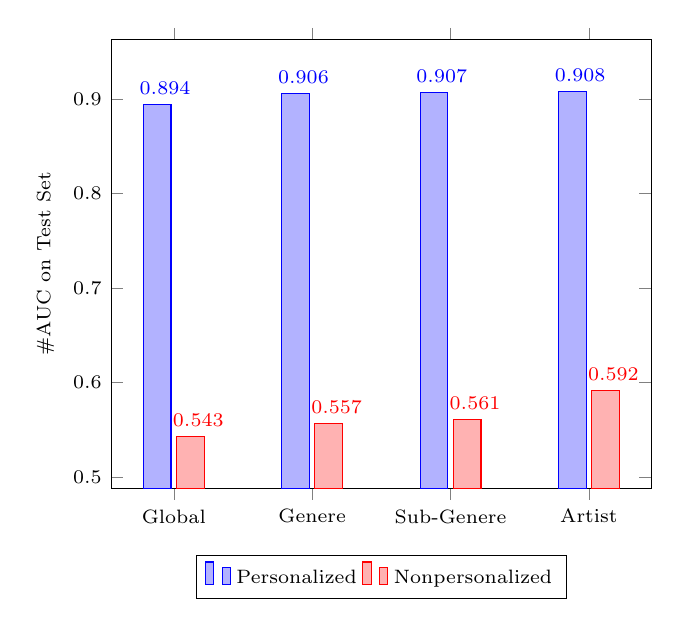
\begin{tikzpicture} 
\begin{axis}[ ybar, enlargelimits=0.15, legend style={at={(0.5,-0.15)}, anchor=north,legend columns=-1}, 
/pgf/number format/precision=5,
font=\scriptsize,
ylabel={\#AUC on Test Set}, 
symbolic x coords={Global,Genere,Sub-Genere,Artist}, 
xtick=data, nodes near coords, nodes near coords align={vertical},
every node near coord/.append style={xshift=0.1cm}  
 ]
 \addplot coordinates {(Global,0.894) (Genere,0.906) (Sub-Genere,0.907)(Artist,0.908)};
 \addplot coordinates {(Global,0.543) (Genere,0.557) (Sub-Genere,0.561)(Artist,0.592)};
  \legend{Personalized,Nonpersonalized}
   \end{axis}
    \end{tikzpicture}
    \caption{Groove Music Dataset}
 \end{figure}
 




%\begin{figure}[H]
\centering

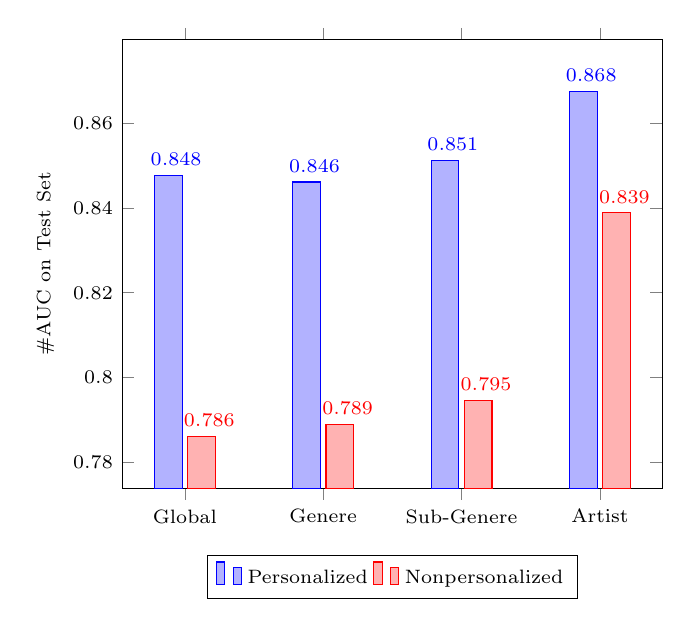
\begin{tikzpicture} 
\begin{axis}[ ybar, enlargelimits=0.15, legend style={at={(0.5,-0.15)}, anchor=north,legend columns=-1}, 
/pgf/number format/precision=3,
font=\scriptsize,
ylabel={\#AUC on Test Set}, 
symbolic x coords={Global,Genere,Sub-Genere,Artist}, 
xtick=data, nodes near coords, nodes near coords align={vertical},
every node near coord/.append style={xshift=0.1cm}  
 ]
 \addplot coordinates {(Global,0.847712777) (Genere,0.846150903	) (Sub-Genere,0.851292881)(Artist,0.867522546)};
 \addplot coordinates {(Global,0.786095642) (Genere,0.788843283) (Sub-Genere,0.794526999)(Artist,0.838879171)};
  \legend{Personalized,Nonpersonalized}
   \end{axis}
    \end{tikzpicture}
    \caption{30 Music Dataset}
 \end{figure}
 



%\paragraph{Effect of Features on Accuracy}
%\begin{figure}

\centering
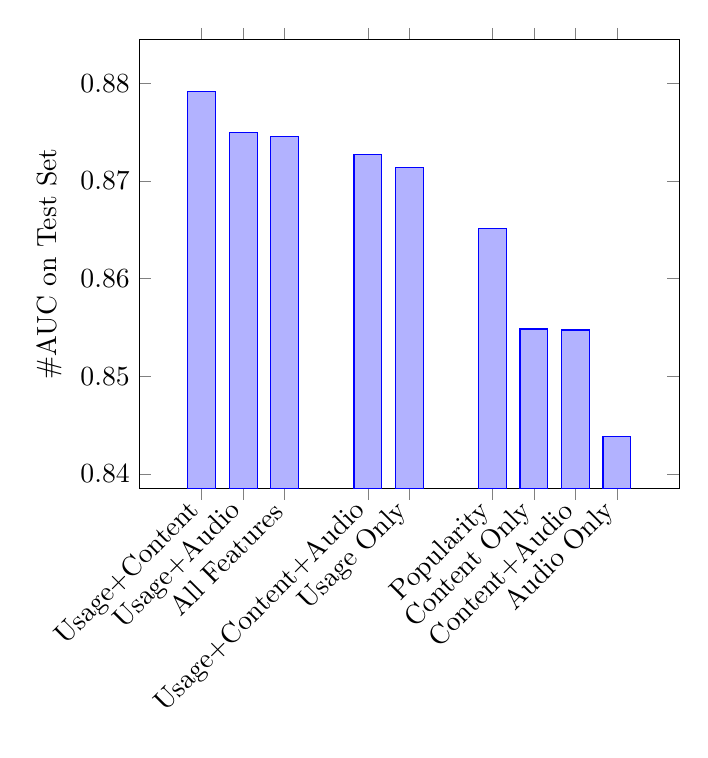
\begin{tikzpicture}
\begin{axis}[ ybar, enlargelimits=0.15, legend style={at={(0.5,-0.15)}, anchor=north,legend columns=-1},
ylabel={\#AUC on Test Set},
symbolic x coords={Usage+Content, Usage+Audio,All Features, ,Usage+Content+Audio, Usage Only, ,Popularity,  Content Only,   Content+Audio,Audio Only},
xtick=data,  nodes near coords align={vertical}, 
x tick label style={rotate=45,anchor=east}
]
 \addplot coordinates {(All Features,0.874533669) (Audio Only,0.843854506)(Content+Audio,0.854736259) (Usage Only, 0.871321339) (Content Only,0.854838861) (Usage+Audio,0.874955404) (Usage+Content,0.879144173)(Popularity,0.865104775)(Usage+Content+Audio,0.872677779)};
 
   \end{axis}
    \end{tikzpicture}
    \caption{Accuracy according to feature group}
    \label{FeaturesFig}
    \end{figure}


\begin{figure}
\scalebox{0.9}{
\begin{tikzpicture}
\begin{axis}[ 
only marks,
ymode=log,xmode=log,
ylabel={Number of Artists},
xlabel={Number of Usage Points}]
\addplot table [x=NumUsagePoints, y=Count, col sep=comma] {histogramOfArtistUsage.csv};


\end{axis}
\end{tikzpicture}}
\caption{A log-log plot of the histogram of usage points for artists in the groove catalog. The large majority of artists have very few observed usage points.}
\label{artistUsageHistFig}
\end{figure}
\input{figs/GenreScatter}

We also considered the contribution of the different feature groups defined in Section~\ref{sec:Features}. To this end we trained the model, using the Groove Music dataset, on each subset of the features separately and evaluated the AUC. Note that for this analysis we used a subset of the data for which no features had missing values. 
%{\bf Usage Features (UF):} These features are derived using collaborative filtering techniques and capture similarity between tracks based on consumption behavior\\
%{\bf Acoustic Audio Features (AAF):} Features based on acoustic audio signals.\\
%{\bf Meta-Data Features (MDF):} Features based on the meta-data features (e.g. "easy-listening", "nineties").\\
%{\bf Popularity Features (PF):} These features simply encode the prevalence of each track in the dataset.\\

Table~\ref{tab:features_AUC} summarizes the  results of this analysis. Using only usage features results in the highest AUC score, followed by popularity, meta-data and acoustic audio features, respectively. Although usage features perform well on their own, we get additional benefits from using other types of features. This is especially relevant when we consider ``cold" artists that have little usage information available. These artists are by far the majority of those appearing in the catalog as can be seen in the histogram (computed over a subset of usage data) shown in Figure~\ref{artistUsageHistFig}.  Furthermore, the importance of usage features in relation to other features varies across the domain taxonomy. Figure~\ref{GenreScatterFig} illustrates this variance. The figure shows that geners such as \textit{Classical} and \textit{Jazz} rely (relatively) much more on audio features and less on usage features than genres such as \textit{Spoken Word} and \textit{Hip Hop}.


\begin{table}[h!]
\begin{center}
	\begin{tabular}{|c|c|c|c|c|c|}
		\hline
		 & {\bf AAF} & {\bf MDF} & {\bf PF} & {\bf UF} & {\bf All}\\ 
		\hline
		 {\bf AUC} & 0.843  & 0.855 & 0.865 & 0.871 & 0.874\\ 
		\hline
	\end{tabular}
	\vspace{-0.4cm}
\end{center}
\caption{AUC achieved by training only on a subset of features on the Groove Music prediction dataset. Feature groups are defined in Section~\ref{sec:Features}}
\label{tab:features_AUC}
\end{table}



% [NK] - This explanations may belong in the features section but not here.
%In some cases, features were missing due to unavailability of data. Normally, we applied zero imputation whenever a feature is missing for a given context. For this experiment, we discarded examples that had missing values in any of the features.

% [NK] - I don't think this sentence is true.
%Apparent is that AUC values are similary for the various feature groups, indicating low variance. This implies, that the different feature groups contain some redundancy in the information they encode. 

% [NK] - This observation does not contribute to the paper. We need to remove it and remove all the groups that outperm  "All Features":
%This also explains the out-performance of the entire feature set by particular subsets of features, perhaps due to a bias variance tradeoff, i.e, overfitting. This phenomenon was not observed on training-set AUC.






%Further, it is interesting to note that the single feature groups for usage and popularity outperform the single feature groups for content and audio. This is especially noteworthy when considering that audio and content features are significantly more expensive to produce in this domain.


\begin{figure}
\scalebox{0.9}{
\begin{tikzpicture}
\begin{axis}[ legend style={at={(0.7,0.325)}, anchor=north,legend columns=-1},
ylabel={AUC},
xlabel={Cumulative amount of data in training set}]
\addplot table [x=index, y=artist2, col sep=comma] {coldnessData.csv};
\addplot table [x=index, y=user, col sep=comma] {coldnessData.csv};
\legend{Artist,User}

\end{axis}
\end{tikzpicture}}
\caption{A cumulative plot illustrating the effect of Artist/User coldness on test AUC. The AUC is plotted for all Artists/Users with at least $x$ labeled data points in the training set.}
\label{coldnessFig}
\end{figure}
In recommendation systems the cold  user/item problem describes the difficulty of
providing recommendations for users/items with little to no previous interaction with the system. 
Figure \ref{coldnessFig} plots the AUC on the Groove Music dataset as a function of the amount of data available for users and artists, respectively. The plot is cumulative e.g., at value $10$ along the X-axis all users / artists with at most $10$ training examples are considered. AUC levels are significantly lower for cold users but quickly improve as the number of training examples increases. This trend is another indication of the importance of personalized information. In contrast to users, there is almost no change in artists' AUC values per different number of observations, and even artists with zero training examples show high AUC values.
This is enabled due to the models use of the domain taxonomy to mitigate the cold artist problem. %The representation of  other artists in the same genre and sub-genre is used in order to allow accurate prediction for artists that have not been at all observed in the training data. 

%We can see that very ``cold" users have dramatically worse predictions than overall. However, as users with more data become available the accuracy quickly increases. This indicates that ``warmer" users contain predictable patterns that the model is able to harness. Artists, on the other hand, are not as sensitive to ``coldness". This is mainly because the semantic hierarchy utilized in our model allows us to generalize the representation of ``cold" artists using other artists in the same genre and sub-genre. Collectively, these results indicate that we are able to generalize artists by pooling data at lower resolution according to the semantic hierarchy.


\GL{I'm not at all sure about this section, firstly the figure does not translate to black and white and is too small when printed. Furthermore, if artists from the same or similar genres are not close, then what exactly is the claim?} \noam{I think I got an explanation:}
Finally, Figure~\ref{tSNEfig} provides an illustration of artist parameters using a t-SNE embedding \cite{Maaten2008} of artist parameter mean values from the Groove music dataset. 
%The figure shows a rich manifold with mixing between artists of several genres. 
Note that proximity in this plot is determined by similarity in the parameters of the learning model. Namely, it does not necessarily reflect ``musical similarity'', but instead it indicates similarity in the importance of the contextual features. The fact that many artists of the same genre do not cluster together supports the model's underlying assumption from Section~\ref{sec:Introduction} that different considerations needs to be applied when generating their playlists. It also suggests that priors at the genre level alone are too coarse and must be broken down to their sub-genres. 

\begin{figure}[h]
	\vspace{-0.2cm}
	\scalebox{0.3}{
		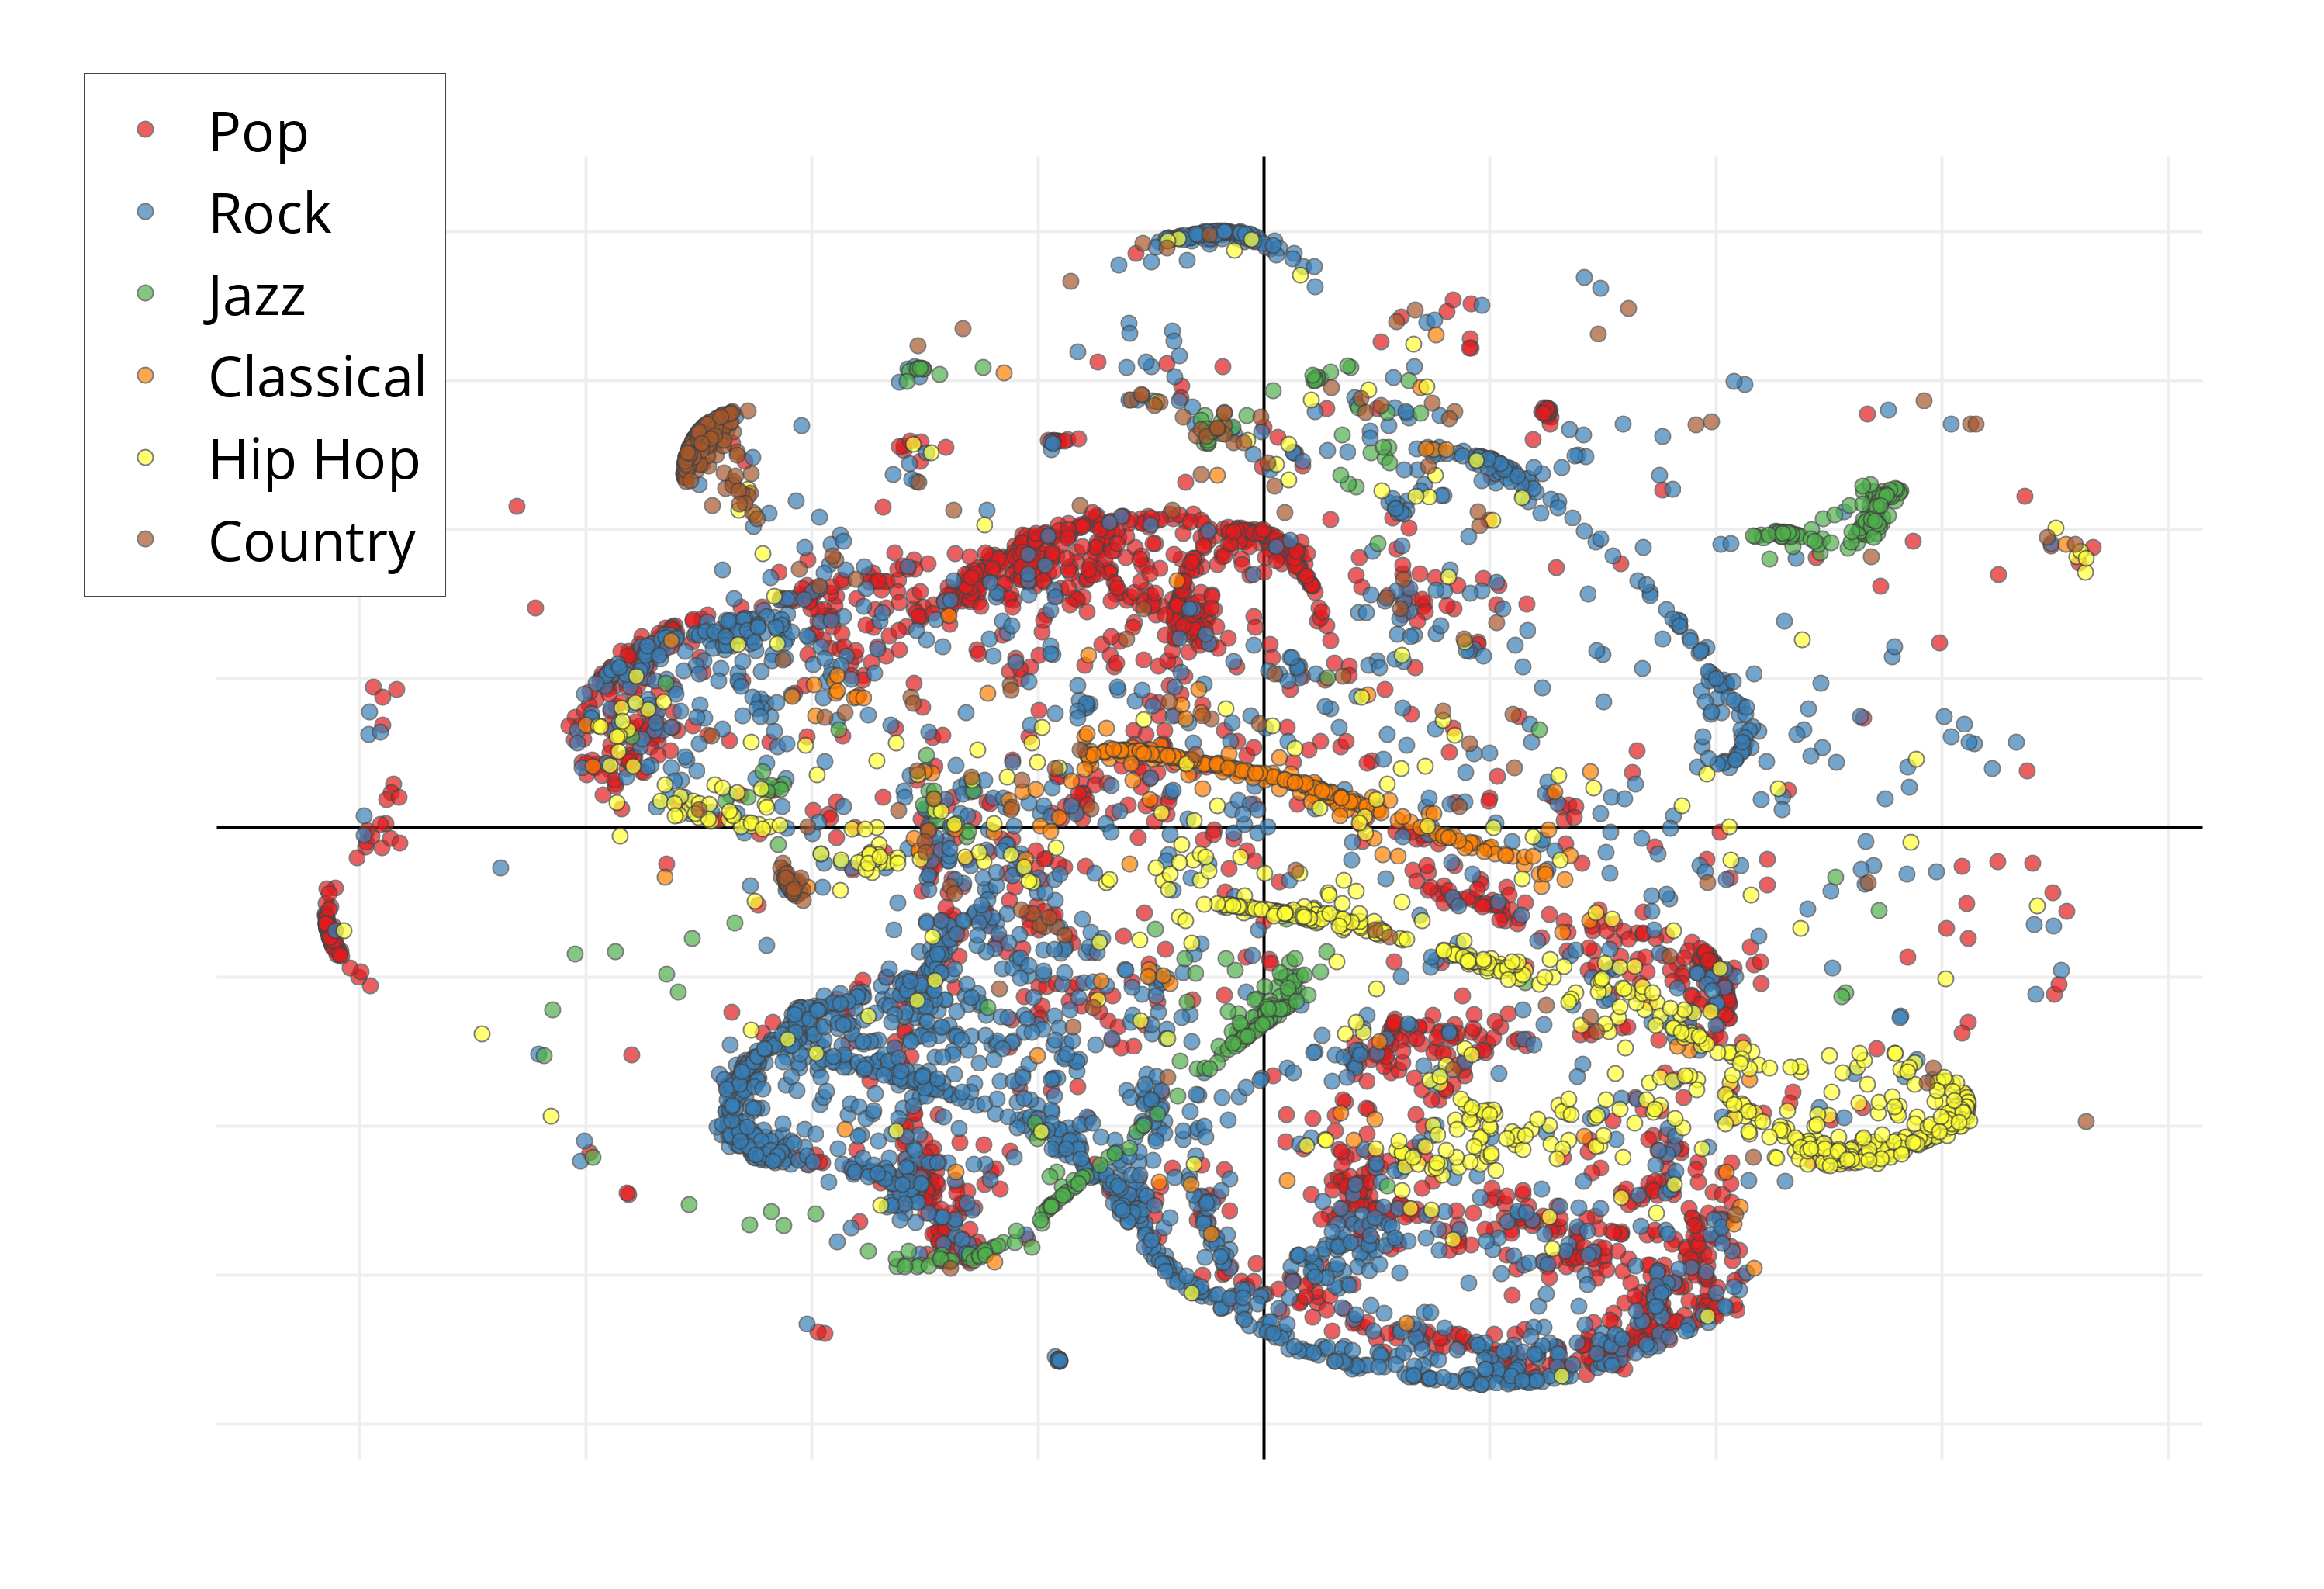
\includegraphics{figs/tSNEfig.png}
	}		
	\vspace{-0.8cm}
	\caption{tSNE embedding of artist parameters. The figure shows a complex manifold that could not be captured by modeling higher levels of the taxonomy alone.}
	\label{tSNEfig}
%	\vspace{-0.3cm}
\end{figure}
 \GL{Doesnt the setup of the model ensure this behavior? Not sure this justifies any assumptions, more like reflects the assumptions of our model IMO. } 

%We present this figure as further evidence that the learned parameters capture inherent semantics in the domain \GL{this final sentence is problematic, how do we see this from the figure?} \noam{Agree.}.

\subsection{Anecdotal Results}

\begin{table}

\centering
\scalebox{0.5}{
\begin {tabular}{lll}%
\\%
\textbf {Track Title} & \textbf {Artist Name} & \textbf {Album Name}\\
 \midrule \multicolumn {3}{c}{\textbf {Artist Seed: Rihanna (Pop Singer)}} \\ 
 \midrule Yeah, I Said It&Rihanna&ANTI\\%
Birthday&Katy Perry&PRISM\\%
She Will Be Loved&Maroon 5&Songs About Jane\\%
I'm Real&Jennifer Lopez&J. Lo\\%
Yeah! (feat. Lil' Jon \& Ludacris)&Usher&Confessions\\%
\midrule \multicolumn {3}{c}{\textbf {Artist Seed: Wes Montogomery (Jazz Guitarist)}} \\ \midrule Bumpin' On Sunset&Wes Montgomery&Wes Montgomery: Finest Hour\\%
The Natives Are Restless Tonight&Horace Silver&Song For My Father\\%
I Remember Clifford&Lee Morgan&The Ultimate Collection\\%
Gee Baby, Ain't I Good To You&Kenny Burrell&Midnight Blue\\%
West Coast Blues&Wes Montgomery&The Jazz Effect - Wes Montgomery\\%
\midrule \multicolumn {3}{c}{\textbf {Artist Seed: Itzhak Perlman (Classical Violinist)}} \\ \midrule Il Postino: Theme (Instrumental)&Itzhak Perlman&Cinema Serenade\\%
Brahms: Hungarian Dance No.5&Nicola Benedetti&The Violin\\%
Violin Concerto No. 2 in E Major ..&Joshua Bell&Bach\\%
Piezas Caracteristicas, Op. 92&John Williams&The Ultimate Guitar Collection\\%
Adagio for Strings&Leonard Bernstein&Barber's Adagio ...\\\bottomrule %
\end {tabular}%
}
\caption{ Anecdotal results: shows the top 5 tracks in the playlist generated for several seed seed artists.} 
\label{anecdotalResultsTable}
\end{table}

To give a flavor of the type of output generated by the proposed approach Table \ref{anecdotalResultsTable} shows the top five tracks in the playlist for three very different seed artists. Notably, using the \textit{Pop} star \textit{Rihanna} as a seed results in a playlist composed of tracks by other \textit{Pop} artists which do not necessarily sound similar to \textit{Rihanna}. For the \textit{Jazz} and \textit{Classical} seed artists, we see that the playlist is not only composed of tracks from the same genre of the artist, but further many tracks include instrumentation similar to that of the seed artist. These playlists are generated by a variant of the algorithm proposed in this work which currently powers the Microsoft's \textit{Groove Music} service.



\GLw{Removed section on AB Testing...}
%\subsection{Online A/B Testing}
%We performed an A/B experiment comparing a variant of the model described above with Groove's previous playlist algorithm. The experiment was conducted by randomly assigning users to buckets and measuring online metrics designed to quantify user satisfaction and engagement. Specifically, we consider \textit{Average Session Length} (ASL), and \textit{User Average Skip Ratio} (UASR). ASL is the listening time elapsed in a single radio session, averaged over all such sessions. UASR is a the ratio of skipped tracks to tracks that were played to completion averaged over all users. The approach in this paper was able to outperform the baseline on both metrics showing an increase of $4.21\%$ in ASL and a $5.76\%$ decrease in UASR.  


%\begin{table}[h]
%\centering
%\begin{tabular}{|c|c|c|}
% \hline
%  KPI & Improvement & P-value \\
% \hline
% ASL & $4.21\%$ & $0$ \\
% \hline
% UASR & $5.76\%$ & $0$\\
% \hline
%\end{tabular}
%    \caption{This table shows the improvement and p-value per measured KPI.}
%    \label{tabel:kpis}
%\end{table}

%\subsection{Anecdotal Comparison}
%
%\begin{table}[H]
%\centering
%\begin{tabular}{ | l | l |l| }
%
%  \hline			
%  Our Algorithm & EchoNest & Last.FM \\
%  \hline
%  Madonna & Shlomo Artzi & John Coltrane\\
%  Cher &  &  \\
%    \hline
%\end{tabular}
%    \caption{Seed Artist:Kylie Minouge}
%\end{table} 




